% ---------------------------------------------------------------
% seccoes/decisao.tex — Processo de decisão e explicação
% ---------------------------------------------------------------

\chapter{Processo de decisão e explicação}\label{sec:5}

\section{Fluxograma de decisão}\label{sec:5.1}

A Figura~\ref{fig:4} representa o ciclo de raciocínio, repetido a cada 100 ms. Em cada ciclo, as regras são avaliadas por fases, cuja ordem é imposta por uma meta-regra. Na fase de perceção, as leituras dos sensores são convertidas em factos que descrevem a situação, como \emph{«peão na passadeira»} ou \emph{«TTC baixo»}. Na fase de decisão, cada regra cujas condições se verificam não executa diretamente uma ação, apenas a propõe. Se nenhuma regra de decisão for ativada, a fase de recurso garante que existe sempre uma ação como, por exemplo, manter a velocidade ou retomar a marcha. No fim do ciclo, todas as propostas são comparadas e é escolhida a ação a executar. Como a escolha é feita apenas no fim, depois de recolhidas todas as propostas, a ordem pela qual as regras disparam não altera o resultado. Neste sentido, a ação final é composta por duas decisões independentes: a decisão de velocidade (acelerar, travar ou parar) e a decisão de via (manter, mudar ou regressar à direita).

Na decisão de velocidade, uma proposta de emergência ou de paragem obrigatória (prioridade 60 ou superior) sobrepõe-se a todas as outras. Ganha a de maior prioridade e, em caso de empate, a de menor velocidade. Se outra regra exigir uma velocidade ainda mais baixa, mantém-se a ação escolhida, mas com essa velocidade. Abaixo desse nível, as propostas de prioridade 50, 40 e 20 funcionam como limites máximos de velocidade. Como o veículo tem de os respeitar todos ao mesmo tempo, adota-se o mais baixo; as propostas de prioridade 30 e 10 dão apenas a velocidade de base quando nenhum teto é inferior, pelo que nenhuma regra consegue levar o veículo acima do limite legal por ter uma prioridade maior (Figura~\ref{fig:5}). No que diz respeito à decisão de via (Figura~\ref{fig:6}), ganha a proposta de maior prioridade e, em empate, regressar à direita vence mudar de via, que vence manter a via. No entanto, uma travagem de emergência nunca dá origem a uma avaliação de manobra: as duas decisões são tomadas em separado e, em caso de conflito, a travagem prevalece. No fim do ciclo, a decisão e o destino de todas as propostas ficam registados e são enviados para a interface, que é o último passo da Figura~\ref{fig:4}.

\begin{figure}[H]
\centering
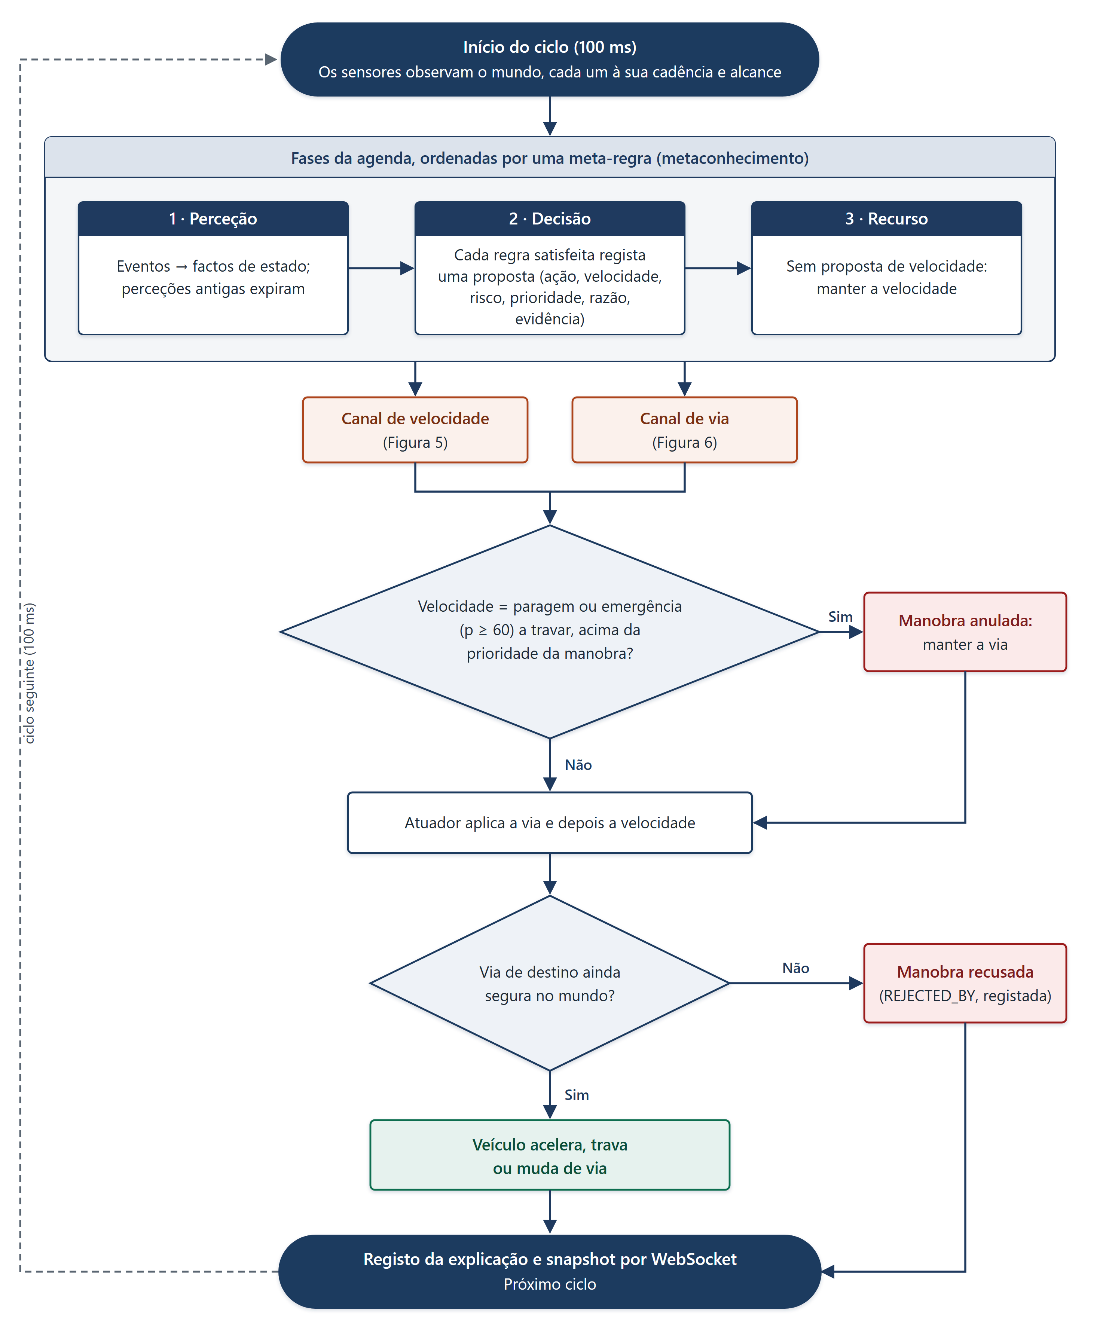
\includegraphics[width=0.79\linewidth,height=0.80\textheight,keepaspectratio]{figuras/fig04_fluxograma_de_inferencia_e}
\caption{Fluxograma de inferência e decisão em cada ciclo de 100 ms}\label{fig:4}
\end{figure}

As Figuras~\ref{fig:5} e~\ref{fig:6} detalham, para cada canal, as perguntas pela ordem de importância. A travagem de emergência está no ramo da velocidade e nunca passa pela pergunta «a manobra é permitida?».

\begin{figure}[H]
\centering
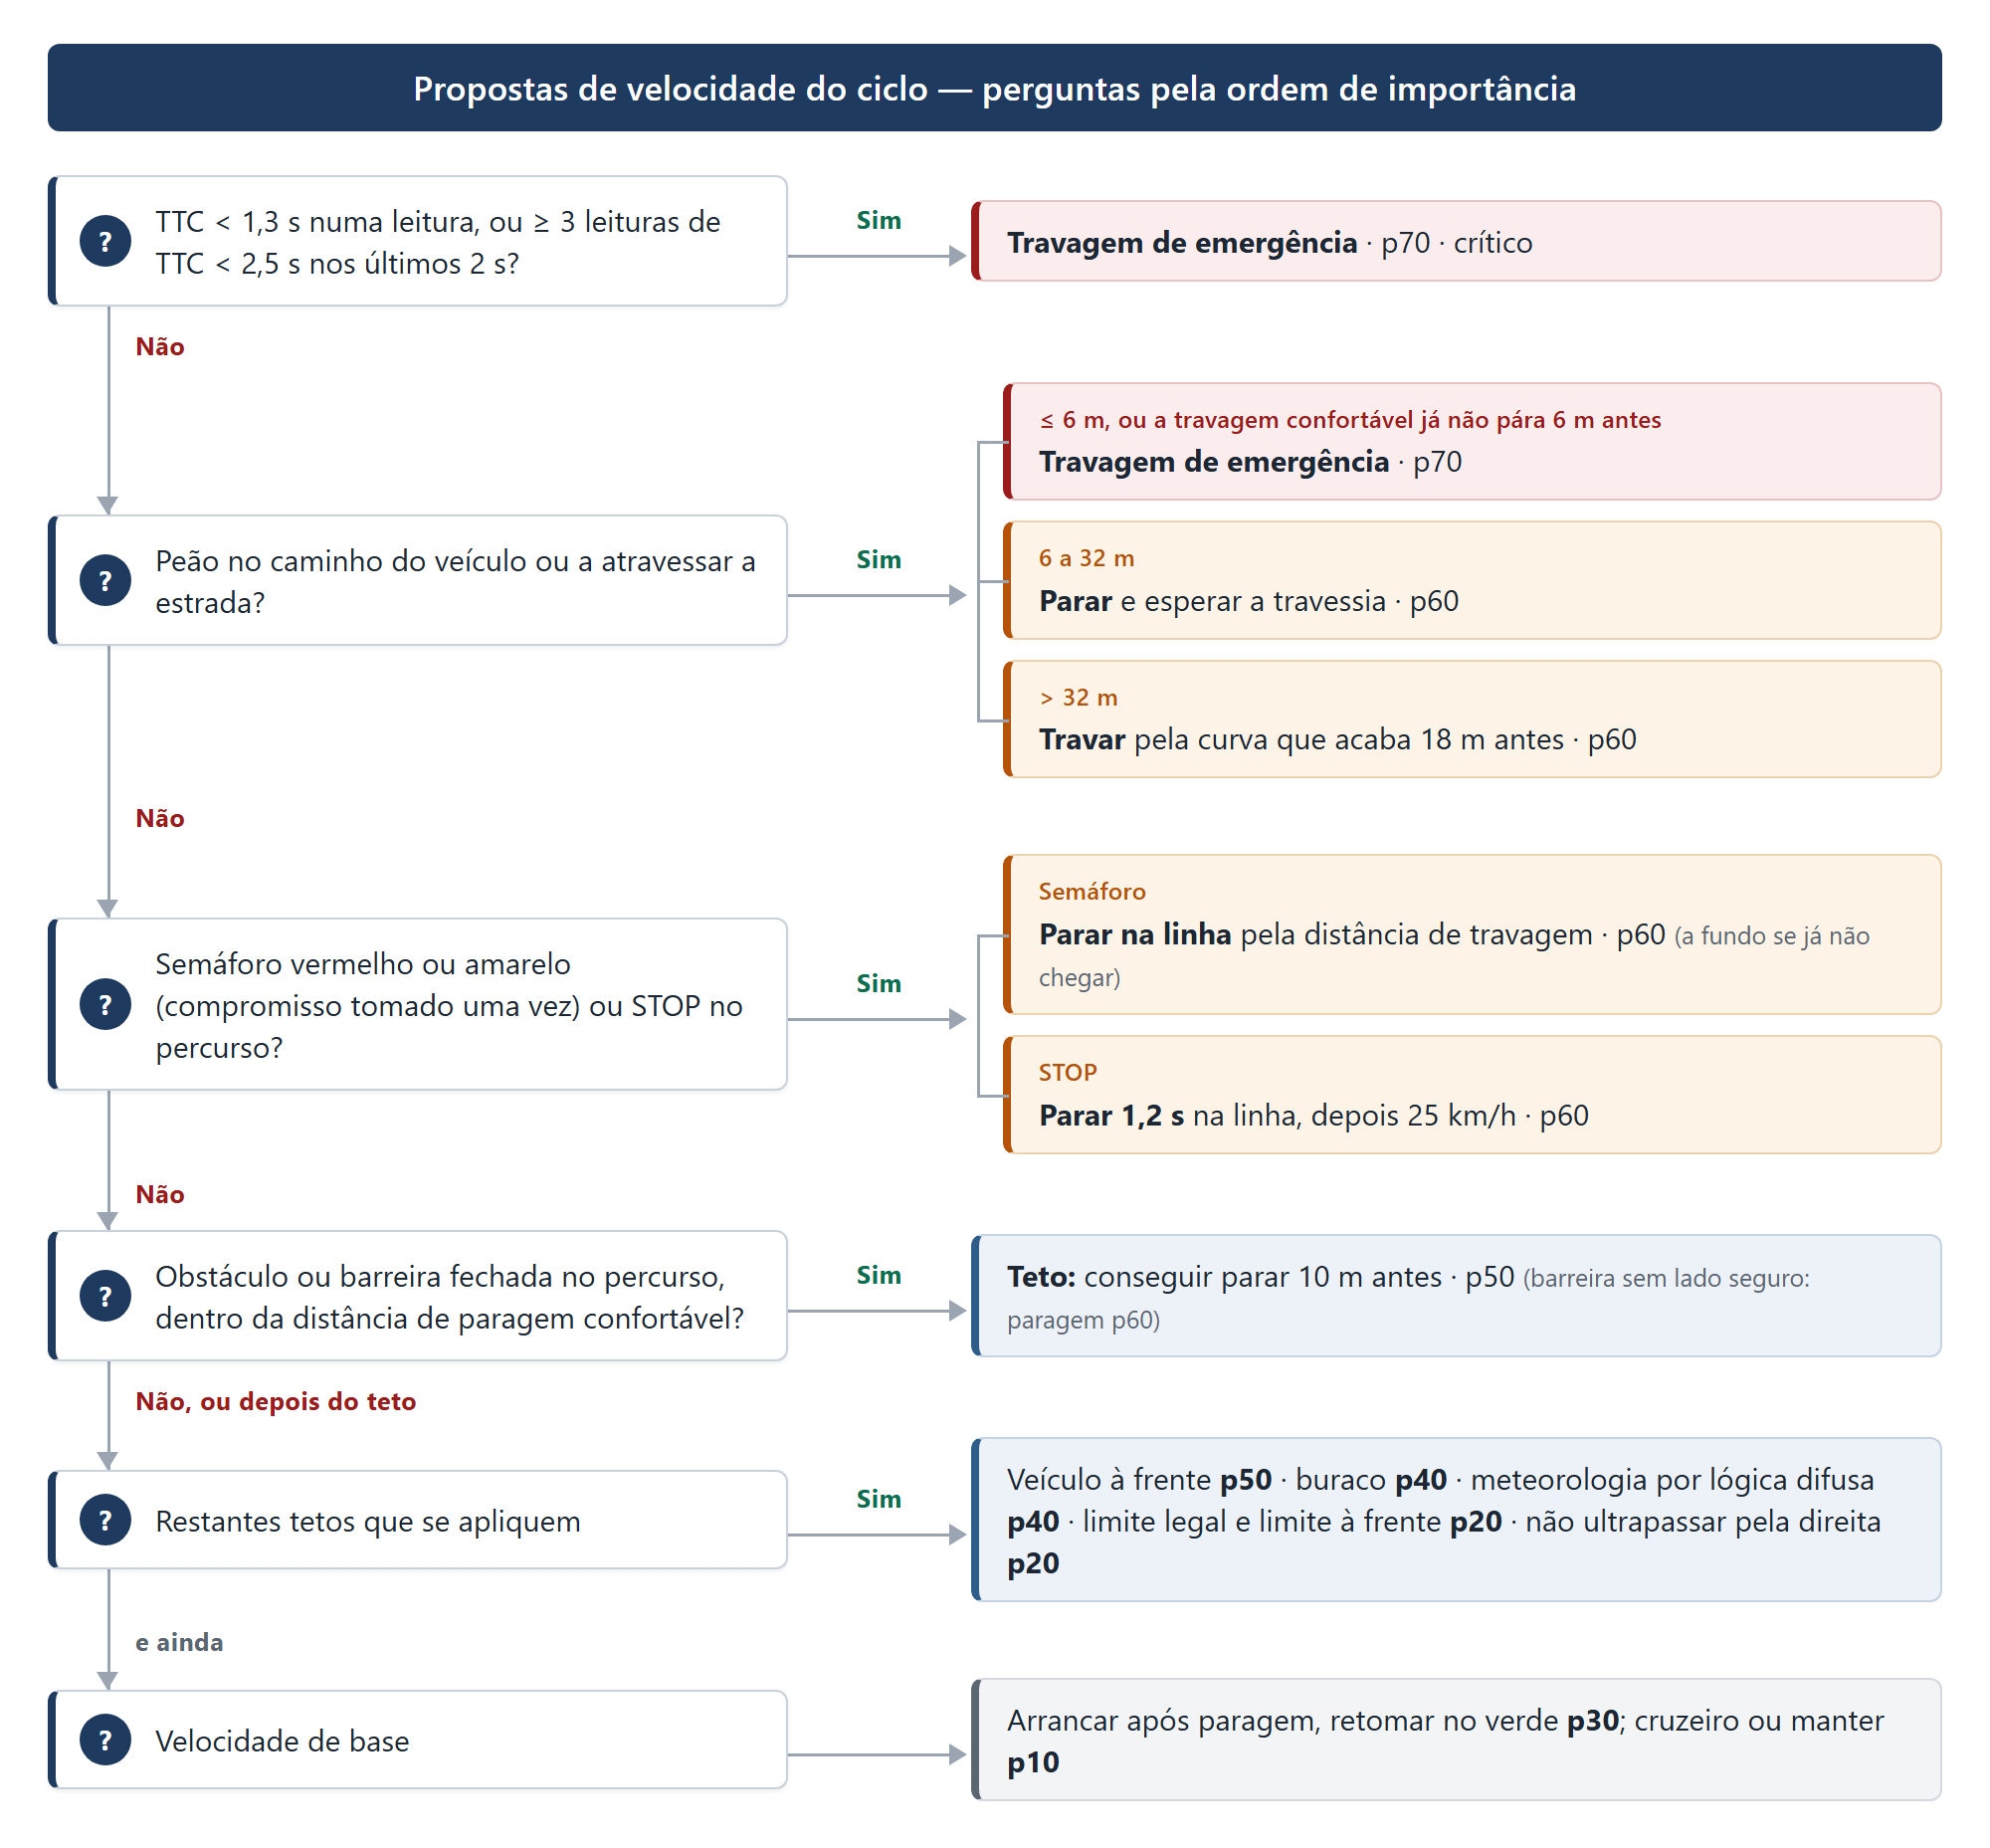
\includegraphics[width=\linewidth,height=0.80\textheight,keepaspectratio]{figuras/fig05_canal_ramo_de_velocidade}
\caption{Canal/ramo de velocidade: perguntas pela ordem de importância e decisão}\label{fig:5}
\end{figure}

No que diz respeito à arbitragem/decisão, se houver uma proposta com p>=60, vence a de maior prioridade e, em caso de empate, a de menor velocidade; um teto mais baixo limita-lhe a velocidade. Caso contrário, cumpre-se o teto mais baixo; a base só vale se nenhum teto for inferior. As restantes propostas ficam registadas como LOST\_TO.

\begin{figure}[H]
\centering
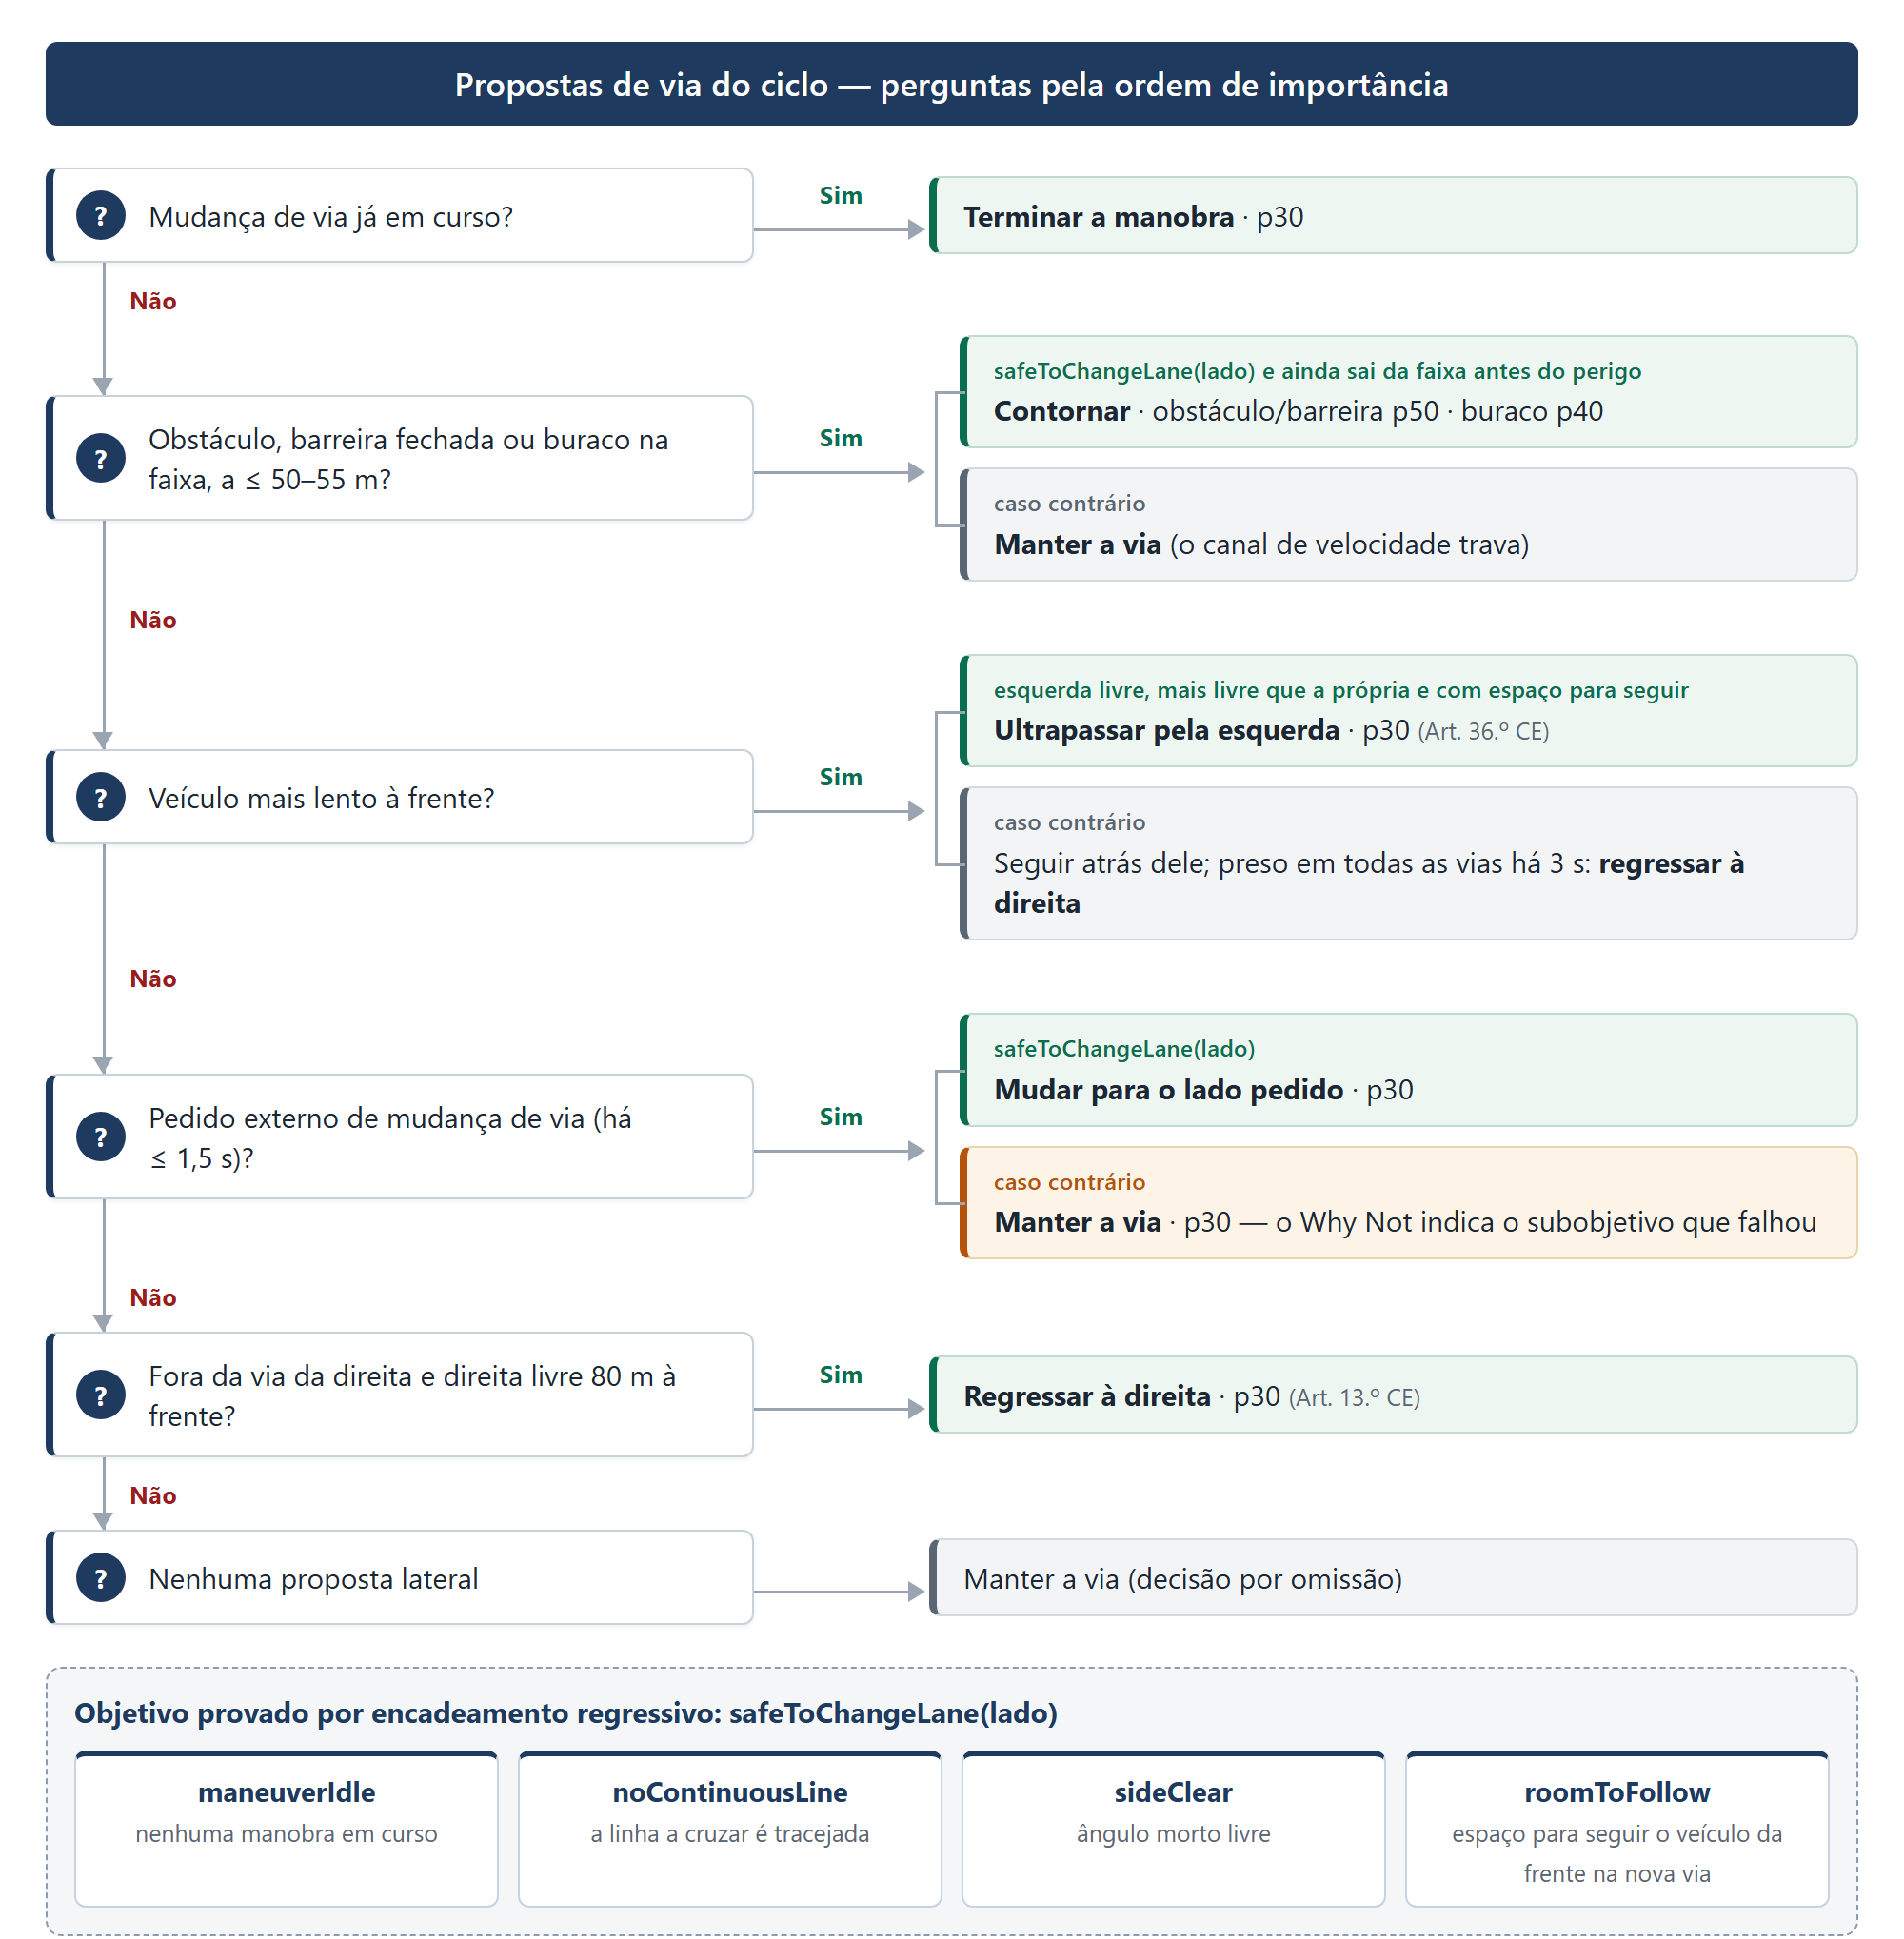
\includegraphics[width=\linewidth,height=0.80\textheight,keepaspectratio]{figuras/fig06_canal_de_via_e_objetivo_provado}
\caption{Canal de via e objetivo provado por encadeamento regressivo}\label{fig:6}
\end{figure}

O canal da via é independente do ramo de velocidade. Neste caso, em situação de empate, vence a proposta de maior prioridade, sendo que regressar à direita > mudar de via > manter a via. Uma manobra é anulada, ou seja, o veículo mantém-se na via inicial, quando a velocidade é uma paragem ou emergência a travar, de prioridade superior à da manobra.

\section{Fluxograma completo}\label{sec:5.2}

As Figuras~\ref{fig:4} a~\ref{fig:6} resumem o processo de decisão e a Figura~\ref{fig:7} apresenta o fluxograma do sistema, por inteiro, em que cada ciclo se repete por 100ms. Para facilitar a leitura, o fluxograma, foi dividido em zonas. As zonas de A a E pertencem ao ramo da velocidade e as zonas F e G ao ramo da via, e a zona G termina com a tomada de decisão.

Este fluxograma deve ser lido como uma ordem de importância e não como uma sequência de execução, uma vez que no \emph{Drools}, todas as regras cujas condições se verificam disparam no mesmo ciclo e registam a sua proposta. A decisão descrita na Secção~\ref{sec:5.1} escolhe depois a proposta vencedora. De seguida, são apresentadas as zonas A, D e G. As restantes podem ser consultadas no Anexo B.

\begin{landscape}
\begin{figure}[H]
\centering
\includegraphics[width=\linewidth,height=0.82\textheight,keepaspectratio]{figuras/fig07_fluxograma_completo_do_processo}
\caption{Fluxograma completo do processo de decisão, dividido em zonas}\label{fig:7}
\end{figure}
\end{landscape}

\textbf{Zona A – Emergência e peões (Figura~\ref{fig:12}). }É a primeira zona, porque trata as situações em que está em causa uma colisão. Uma única leitura de TTC inferior a 1,3 s, ou três leituras inferiores a 2,5 s nos últimos 2 s, dá origem a uma travagem de emergência. Se houver um peão no caminho do veículo, a resposta depende da distância. Um obstáculo grave a 8 m ou menos, na via em que o veículo circula, também dá origem a uma emergência, termina diretamente na decisão de velocidade e nunca passa por uma avaliação de manobra.

\textbf{Zona B – Semáforos (Figura~\ref{fig:13}). }Perante um semáforo vermelho, o veículo compara a distância à linha com a distância de que precisa para parar: 0,5 s de reação, mais a travagem, mais 18 m. Se estiver longe, continua. Se estiver na zona de transição, deixa de acelerar. Se já estiver dentro da distância de travagem, trava com conforto (2,8 m/s²) e para na linha, ou trava a fundo quando a travagem confortável o desloca a mais de 2 m para lá da linha. No amarelo, a decisão de parar ou prosseguir é tomada uma única vez, para evitar que o veículo hesite e trave a meio do cruzamento. No verde, o veículo segue ou volta a arrancar.\par \par \textbf{Zona C – STOP, barreiras e obstáculos (Figura~\ref{fig:14}). }No sinal STOP, o veículo para na linha e só avança, a 25 km/h, depois de estar parado pelo menos 1,2 s, o que garante a paragem completa exigida pelo Código da Estrada. Face a uma barreira fechada ou a um obstáculo dentro da distância de paragem segura, o veículo trava para conseguir parar 10 m antes. No caso da barreira, se for seguro mudar de via, essa travagem dura apenas até a mudança o tirar do caminho. Se for preciso travar a mais de 3,1 m/s², a travagem passa a ser a fundo.

\textbf{Zona D – Limites, veículo à frente e chuva (Figura~\ref{fig:15}). }Esta zona dá origem a tetos de velocidade (prioridades 50 e 20), aplicadas em simultâneo. O veículo respeita o limite em vigor e começa a abrandar a tempo de chegar ao sinal seguinte já com o novo limite, ao travar a 2,0 m/s². Com um veículo à frente, para cerca de 12 m atrás se este estiver parado. Se estiver em movimento, abranda até 3 km/h abaixo dele, acompanha a sua velocidade ou abranda apenas o necessário, conforme a distância. Com pouca aderência, essa distância duplica. O veículo não ultrapassa pela direita um veículo mais lento na via da esquerda. Com chuva, duas leituras de TTC inferiores a 3 s em 2 s levam o veículo a travar até 15 km/h.\par \textbf{Zona E – Buracos, meteorologia e velocidade de base (Figura~\ref{fig:16}). }Se não conseguir desviar-se de um buraco, o veículo passa por ele a 30 km/h, e a 20 km/h nos últimos 15 m. Junto a uma barreira aberta, não passa de 35 km/h. Com chuva, visibilidade reduzida ou pouca aderência, a lógica difusa calcula uma velocidade máxima recomendada, entre cerca de 25 e pouco mais de 70 km/h. Só depois de considerados todos os tetos é definida a velocidade de base: arrancar após uma paragem, acelerar a pedido, manter o limite do sinal ou retomar a velocidade de cruzeiro. Se nenhuma regra se aplicar, a fase de recurso mantém a velocidade. Por fim, vale a velocidade mais baixa entre a de base e todos os tetos encontrados, pelo que o veículo nunca ultrapassa o limite legal.

\textbf{Zona F – Via: obstáculos, barreiras e buracos (Figura~\ref{fig:17}). }O ramo referente ao comportamento em via começa por confirmar se uma emergência ou paragem obrigatória está a travar o veículo. Se estiver, o veículo mantém a via, o que garante que nenhuma manobra compete com uma travagem crítica. Uma mudança de via já iniciada é sempre concluída. Perante um obstáculo, uma barreira fechada ou um buraco na via, o veículo contorna-o se for seguro mudar de via e se ainda conseguir sair da via antes de lá chegar. Caso contrário, mantém a via e o canal de velocidade trata da paragem ou da passagem lenta.

\textbf{Zona G – Ultrapassagem, pedidos, regresso à direita e atuação (Figura~\ref{fig:18}). }Atrás de um veículo mais lento, o veículo ultrapassa apenas pela esquerda. Se estiver preso atrás de trânsito lento em todas as vias há pelo menos 3 s, desiste e regressa à direita. Um pedido externo de mudança de via só é aceite se a mudança for segura. Se não for, é recusado e a explicação indica qual das condições falhou. Sem outro motivo para ficar, o veículo regressa à via da direita, uma via de cada vez, como determina o Código da Estrada. As decisões de velocidade e de via juntam-se na atuação. Antes de iniciar uma mudança de via, o atuador volta a confirmar no mundo que a via de destino está livre e que não há linha contínua. Se alguma destas condições falhar, cancela a manobra e abranda 10 km/h. Por fim, ajusta a velocidade com suavidade e começa o ciclo seguinte.

\section{Explicação da decisão}\label{sec:5.3}

Cada decisão responde a três perguntas, todas a partir do que as regras registam e visíveis na interface:

\begin{itemize}
  \item \textbf{\emph{Why: }}a regra vencedora, a razão, a evidência (valores dos factos usados), o risco e a prioridade.
  \item \textbf{\emph{How:}} a linha temporal regista, com instante, cada facto inserido, atualizado ou removido e cada regra disparada, o que permite reconstruir o percurso sensor → evento → facto → regra → decisão.
  \item \textbf{\emph{Why Not: }}todas as propostas do ciclo ficam guardadas com o seu destino (Tabela~\ref{tab:9}).
\end{itemize}

\begin{tabela}{L{\dimexpr0.1865\linewidth-2\tabcolsep\relax}L{\dimexpr0.2988\linewidth-2\tabcolsep\relax}L{\dimexpr0.5128\linewidth-2\tabcolsep\relax}}
\caption{Destinos possíveis de uma proposta}\label{tab:9}\\
\linhacab \cab{\textbf{Estado}} & \cab{\textbf{Significado}} & \cab{\textbf{Exemplo}} \\
\endfirsthead
\linhacab \cab{\textbf{Estado}} & \cab{\textbf{Significado}} & \cab{\textbf{Exemplo}} \\
\endhead
WON & Venceu a arbitragem. & Travagem de emergência (p70) por TTC crítico persistente. \\
\rowcolor{corFundo}LOST\_TO & Perdeu para outra de maior prioridade. & Regras de meteorologia perdem para a emergência. \\
VETOED\_BY & Anulada por uma paragem ou emergência. & Mudança de via, anulada pela travagem de emergência. \\
\rowcolor{corFundo}CAPPED & Venceu, mas com a velocidade limitada por um teto mais baixo. & Paragem obrigatória, com outra regra a exigir velocidade ainda menor. \\
REJECTED\_BY & Recusada pelo atuador por ser insegura. & Mudança de via com a via de destino ocupada ou com linha contínua. \\
\end{tabela}

Como recomendou o perito, o texto de cada explicação é a razão e a evidência registadas pela regra que disparou, e não uma descrição escrita à parte. No fim da viagem a sessão é gravada em JSON, e qualquer decisão pode ser questionada depois sem reavaliar nada. A Secção~\ref{sec:6.4} mostra as três explicações num caso concreto.
